\chapter*{Instalasi Python dan PIP}
\section*{Instalasi Python}

\begin{enumerate}
	\item Setelah selesai mendownload apk anaconda. double klik apk maka akan muncul tampilan sebagai berikut dan pilih next 
	\begin{figure} [h]
	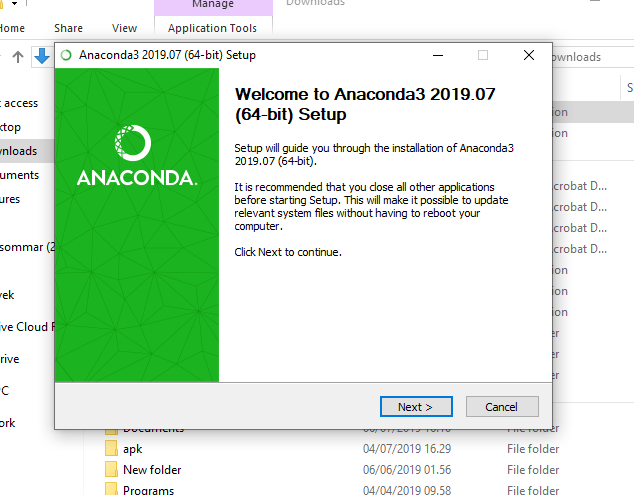
\includegraphics[width=9cm]{section/picpyt/pyt1.png}
	\centering
	\end{figure}
	
	\item lalu akan muncul assignment agreement, setelah membacanya lalu klik "i agree"
	\begin{figure} [h]
	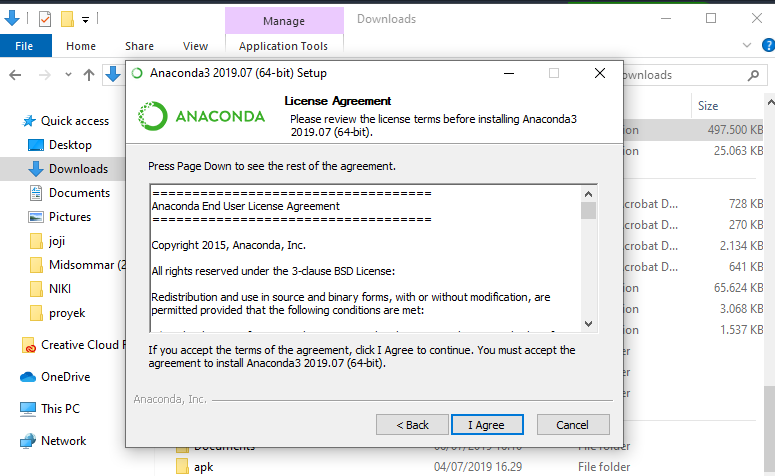
\includegraphics[width=6.5cm]{section/picpyt/pyt2.png}
	\centering
	\end{figure}
	
	\item lalu pilih destinasi folder tempat penginstallan anaconda, lalu pilih next 
	\begin{figure} [h]
	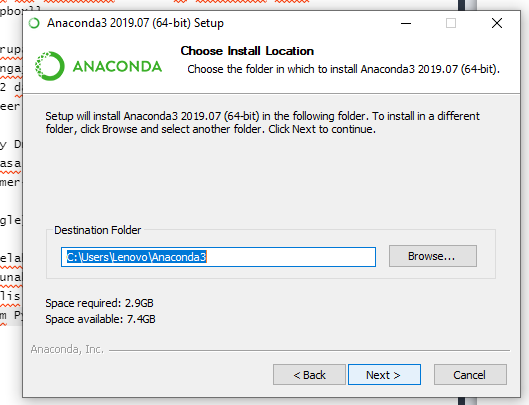
\includegraphics[width=6.5cm]{section/picpyt/pyt3.png}
	\centering
	\end{figure}
	
    \item lalu pilih "just me" sehingga hanya user anda di laptop anda yang bisa menjalankan anaconda 
	\begin{figure} [h]
	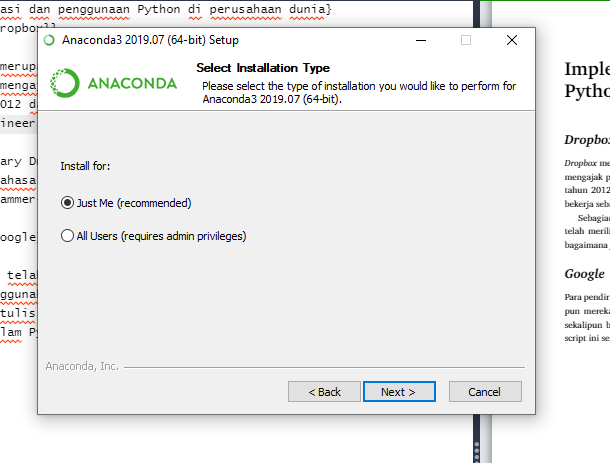
\includegraphics[width=6.5cm]{section/picpyt/pyt4.png}
	\centering
	\end{figure}
	
	\item lalu "Register Anaconda as my default Python 3.7" sehingga beberapa program akan otomatis mendetek Anaconda sebagai Python utamanya
	\begin{figure} [h]
	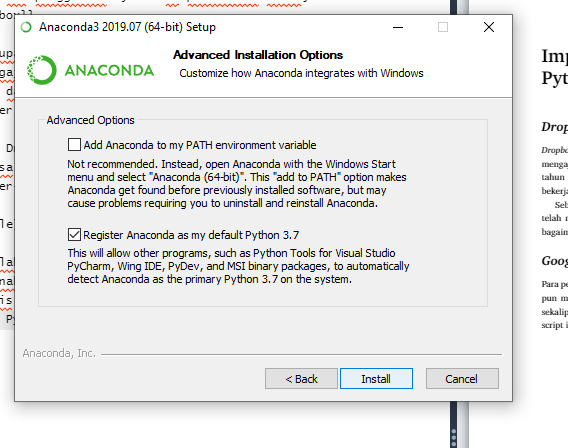
\includegraphics[width=6.5cm]{section/picpyt/pyt5.png}
	\centering
	\end{figure}
	
	\item setelah proses install selesai, maka anaconda sudah terinstall

	

	\end{enumerate}
	
	

